\Chapter{A virtuális kollaborációs tér}

% A fejezet gyakorlatilag a kliens kialakításáról szól.

% Maga a menü, beállítások és egyéb felületi elemek is lehetnek 3D-sek.

\Section{Megjelenítési mód}

{\bf OpenGL, PyOpenGL:}

Az OpenGL egy 2D-s és 3D-s vektor grafikus  API, ami elérhető és támogatott a fő operációs rendszereken (Linux, macOS, Windows) valamint számos programozási nyelvvel kompatibilis.

Az OpenGL pythonnal használható verziója a cross-platform, nyíltforráskodú PyOpenGL. A PyOpenGL zámogatja a GL, GLU és GLUT könyvtárakat.

A program obj kiterjesztésű modellekkel dolgozik, amikhez mtl kiterjesztésű textúrát rendel. 
\begin{itemize}
\item {\bf obj}: Az OBJ (vagy .OBJ) egy geometria-definíciós fájlformátum, amelyet a Wavefront Technologies fejlesztett ki először az Advanced Visualizer animációs csomagjához. A fájlformátum nyílt forrású, ezért más 3D-s grafikus alkalmazások gyártói átvették.
Az OBJ egy egyszerű formátum (ember által is olvasható), ami a 3D geometriát adja meg csupán: a csúcsok helyzetét, az egyes textúra koordináta-csúcsok helyzetét, a csúcsok normálisát (???), az egyes sokszögeket csúcsok listájaként definiáló faces(???), textúre csúcsokat.  
\item {\bf mtl}: Az MTL fájl egy segédfájl, amely a modell anyagainak meghatározását tartalmazza, amelyekhez OBJ fájl hozzáférhet. Az OBJ fájlnak meg kell adnia az MTL fájl nevét. Az MTL fájl az anyagok definícióinak sorrendjét tartalmazza. Mindegyik definíció egy newmtl utasítással kezdődik, amely meghatározza az anyag nevét, majd azon sorok következnek, amelyek megadják az adott tulajdonságokot.
\end{itemize} 


A program fő elemei az ágensek. A model, amit felhasználtam egy császárpingvin. 
\begin{figure}[htp]
    \centering
   	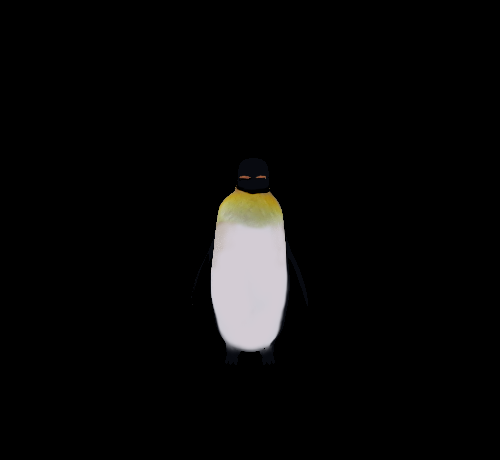
\includegraphics[width=4truecm, height=3truecm]{images/penguin.png}
	\caption{császárpingvin modell}
\end{figure}

A program szinterének fő eleme a kastély modell, ahol maga a jelenet játszódik.\\
\begin{figure}[htp]
    \centering
   	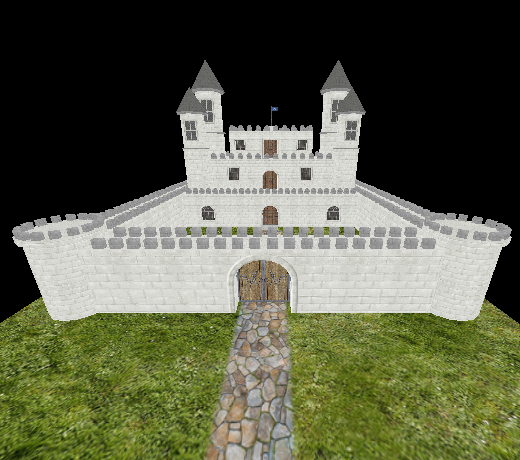
\includegraphics[width=4truecm, height=3truecm]{images/castle.png}
	\caption{kastély modell}
\end{figure}

Felhasználtam továbbá doboz modelleket, amiknek az elmozgatása a feladat.
\begin{figure}[htp]
    \centering
   	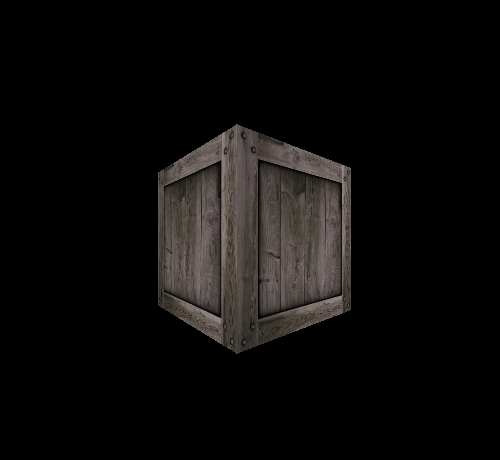
\includegraphics[width=4truecm, height=3truecm]{images/box.png}
	\caption{doboz modell}
\end{figure}

{\bf Fények:}

Az objektumok megjelenítéséhez elengedhetetlenek a megfelelő fénybeállítások.\\

„Az ábrázolandó térrészben uralkodó fényviszonyok leírására az alábbi fényösszetevőket szokásfigyelembe venni:

\begin{itemize}
\item A {\bf környezeti fény} (\texttt{ambient light}) az ábrázolandó térrészben mindenütt jelen lévő, állandó intenzitású fény, amelynek forrása, iránya nem ismert (gondoljunk olyan nappali fényre,amikor a nap a felhők mögött van).
\item A {\bf szórt fénynek} (\texttt{diffuse light}) van iránya, mindig valamelyik fényforrásból jön. Fő jellemzője, hogy az objektumokkal ütközve minden irányba azonos módon és mértékben verődik vissza, tehát teljesen mindegy, hogy milyen irányból nézzük az objektumokat, a hatás csak a fényforrástól, az anyagtulajdonságoktól és a pontbeli normálistól függ.
\item A {\bf tükröző fénynek} (\texttt{specular light}) is van iránya és forrása, és hatása nemcsak az anyag-tulajdonságoktól és a pontbeli normálistól, hanem a nézőponttól is függ. Gondoljunk egy sima felületű fémgömbre, amit erős, koncentrált fénnyel világítunk meg. Megfelelő szögből nézve egy fényes (többnyire fehér) foltot látunk, amelynek mérete és helye a nézőponttól függ, fejünket mozgatva a folt is mozog, mígnem eltűnik.”
\end{itemize}

\Section{Interaktív elemek}

Szintér
A térben mozgatható, interaktív elemek.

Az obj formátum nem támogatja az animációt, ezért minden egyes mozdulatnak külön obj és mtl fájlja készült.
Az animációkat a testvérem készítette el Blender felhasználásával. Az elkészült animációk a következők:
ugrás, séta és a dobozok tolásához a doboz megfodása és elengedése.
 
Fizika megvalósításával kapcsolatban észrevételek.

\Section{Az elemek vezérlése}

{\bf Billentyű, egér funkciók:}\\

Az ágens irányításához (lépés előre, hátra, fordulás, ugrás) a nyíl és a space-t billentyűket használtam fel, a  programból való kilépéshez az „ESC” billentyűt. Továbbá ez egér lehetővé teszi, hogy más szögből lássuk a jelenetet.\\
%Kell valami amivel tollja a dobozt is és ha lesz menü, akkor arra is egy gombot kijelölni!!

{ \bf A felhasznált függvények:}

\begin{itemize}
\item A \texttt{glutKeyBoardFunc()}-nek három paramétere van: \texttt{key} a generált ASCII karakter, az \texttt{x} és \texttt{y} pedig az egér pozíciója abban az időpontban, mikor a billentyű lenyomás történt a \texttt{GLUT} ablakhoz képest. Ezzel a funkcióval csak a kilépéshez szükséges \texttt{ESC} billentyű lenyomás kezelődött le, a nyíl billentyűkhöz és a \texttt{space}-hez egy másik funkció szükséges.
\item A \texttt{glutSpecialFunc()} szükséges speciális billentyűk lenyomásának kezeléséhez,  
aminek szintén három paramétere van, a key, ami egy \texttt{GLUT\_KEY\_*} konstans, és az \texttt{x} és \texttt{y}, amik ugyanazt jelölik, mint az előző esetben, az egér relatív helyzetét az ablakhoz képest.
\item A \texttt{glutMouseFunc()} az egér billentyűinek a lenyomását a  tudjuk nyomon követni, a mozgását pedig a \texttt{glutMotionFunc()}-al vagy a \texttt{glutPassiveMotionFunc()}-al. A glutMotionFunc azt az eshetőséget kezelei le, amikor egy vagy több billentyű lenyomás történt és közben lett mozgatva az egér. A \texttt{glutPassiveMotionFunc()} pedig azt, amikor úgy lett mozgatva az egér, hogy nem lett lenyomva egyetlen egér gomb sem.  
\end{itemize}
